\chapter{Pilotstudie}
\label{sec:pilotstudie}

In diesem Kapitel dokumentiere ich die Durchführung und die Analyse einer Pilotstudie, mit der ich überprüfe, ob das in dieser Arbeit entwickelte Forschungsdesign -- bestehend aus dem Erhebungsinstrument \gls{intermind} und dem dazugehörigen Fragebogen (\cref{sec:entwicklung_app,sec:fragebogenentwicklung}) -- geeignet ist, Daten zu generieren, die sich für eine intersektional-quantitative Analyse nutzen lassen. Zudem begründe ich meine Entscheidung für \gls{i-maihda} als Analyseverfahren und reflektiere dessen Anschlussfähigkeit an eine intersektionale Perspektive.


Als Testfall dient die folgende Überprüfungsfrage:
\begin{quote}
Wie beeinflussen räumliche Umgebungen das situierte (Un\nobreakdash-)Wohlbefinden intersektional positionierter Personen im Alltag?
\end{quote}

Die Frage ist bewusst allgemein formuliert, da sie in dieser Pilotstudie nicht vollständig beantwortet, sondern methodisch erprobt wird. Ziel der Pilotierung ist es, zu untersuchen, ob die erhobenen Daten eine statistische Auswertung grundsätzlich zulassen und welche praktischen, technischen und konzeptionellen Herausforderungen dabei sichtbar werden. In \cref{sec:diskussion} ordne ich anschliessend ein, inwiefern diese Ziele erreicht wurden und welche Schlüsse sich daraus für die Weiterentwicklung des Forschungsdesigns ziehen lassen.

Sämtlicher Analysecode ist im \gls[noindex]{github}-Repository\footnote{\href{https://github.com/lbatschelet/Designing-InterMind}{https://github.com/lbatschelet/Designing-InterMind}} dieser Arbeit verfügbar.

\section{Stichprobe}

Die Datenerhebung fand im Rahmen der einführenden Exkursion \enquote{Recht auf Stadt} im ersten Studienjahr des Bachelorstudiengangs Geographie an der Universität Bern im Mai 2025 statt. Zu Beginn jedes der insgesamt vier Exkursionstage erfolgte eine Einladung zur freiwilligen Teilnahme an der Studie -- beim ersten Termin von mir persönlich, an den folgenden Terminen durch die Exkursionsleitenden. Für jede teilnehmende Person begann die Erhebungsphase mit einer einmaligen Baseline-Befragung und dauerte ab diesem Zeitpunkt sieben Tage.

\subsection*{Demographische Daten aus der Baseline Befragung}

Insgesamt wurden rund \num{80} Personen zur Teilnahme eingeladen. \num{32} davon haben die App heruntergeladen und die einmalige Baseline-Befragung begonnen. \num{8} begonnene, aber nicht abgeschlossene Baseline-Befragungen wurden aus der Stichprobe ausgeschlossen. Die endgültige Stichprobe umfasst somit \num{24} Personen. \cref{tab:kreuztabelle_abs} zeigt die Verteilung von sozialem Geschlecht und Altersgruppe.

\footnotesize
\begin{table}[htb]
    \caption{Kreuztabelle: Soziales Geschlecht und Altersgruppe (absolute Häufigkeiten)}
    \label{tab:kreuztabelle_abs}
    \centering
    \begin{tabular}{lcccS}
        \toprule
        \textbf{Geschlecht} & 16--25 & 26--35 & Keine Angabe & \multicolumn{1}{c}{Gesamt} \\
        \midrule
        Mann & 12 & 2 & 1 & 15 \\
        Frau &  8 & 1 & 0 &  9 \\
        \midrule
        \textbf{Gesamt} & 20 & 3 & 1 & 24 \\
    \end{tabular}
\end{table}
\normalsize
    
  

Die Mehrheit der Teilnehmenden verfügt über eine \emph{Matura oder ein gleichwertiges Abschlusszeugnis} (\num{22}; \SI{92}{\percent}), zwei Personen (\SI{8}{\percent}) besitzen einen Hochschulabschluss. Der überwiegende Teil ist als \emph{Student\genderstern in oder Schüler\genderstern in} erwerbstätig (\num{21}; \SI{88}{\percent}), drei Personen (\SI{12}{\percent}) sind angestellt. Die grosse Mehrheit wurde im gleichen Land geboren, in dem sie derzeit lebt (\num{16}; \SI{68}{\percent}), \num{7} Personen (\SI{28}{\percent}) nicht; eine Person (\SI{4}{\percent}) machte keine Angabe.

Alle Personen gaben keine vorhandene Behinderung an (\num{24}; \SI{100}{\percent}).

Bezüglich der sexuellen Orientierung gaben \num{17} Personen (\SI{68}{\percent}) \emph{hetero} an, jeweils drei (\SI{12}{\percent}) \emph{homosexuell} oder \emph{bisexuell}, und eine Person (\SI{4}{\percent}) \emph{queer}. 

Beim gruppierten Äquivalenzeinkommen entfallen \num{8} Personen (\SI{32}{\percent}) auf die Kategorie \emph{Sehr niedrig}, \num{6} (\SI{24}{\percent}) machten keine Angabe, \num{5} (\SI{20}{\percent}) gehören zur Kategorie \emph{Hoch}, \num{4} (\SI{16}{\percent}) zu \emph{Niedrig} und \num{1} (\SI{4}{\percent}) zu \emph{Sehr hoch}.

Die hier gewählte Darstellung trennt die einzelnen Merkmale bewusst auf, um die Zusammensetzung der Stichprobe transparent zu machen. Methodisch betrachtet widerspricht diese Entzerrung jedoch einem intersektionalen Ansatz, da \glspl[noindex]{identitaetsachse} in isolierte Kategorien zerlegt werden. Die vollständige Übersicht über die Angaben aus der Baseline Befragung ist in \cref{app:appendix_demographics} festgehalten.

\subsection*{Momentaufnahmen}

Insgesamt liegen \num{106} vollständig abgeschlossene Momentaufnahmen vor. Weitere \num{6} begonnene, aber nicht abgeschlossene Momentaufnahmen sind von der Analyse ausgeschlossen. \cref{fig:survey_counts} zeigt die Verteilung der Anzahl abgeschlossener Momentaufnahmen pro Person.

Die Verteilung der Aufenthaltsorte gliedert sich in die in \cref{fig:survey_locations} dargestellten Kategorien. Unabhängig davon sind die Erhebungen zusätzlich als Innen- \gls{bzw} Aussenraum codiert: Praktisch gleich viele Befragungen wurden in Innenräumen ($n=\num{54};\,\SI{51}{\percent}$) wie in Aussenräumen ($n=\num{52};\,\SI{49}{\percent}$) durchgeführt.

Die während der Momentaufnahmen ausgeübten Tätigkeiten sind in \cref{fig:survey_activities} zusammengefasst.

Das soziale Umfeld variiert: Etwa ein Drittel der Befragungen wurden ohne die Anwesenheit anderer Personen durchgeführt ($n=\num{37};\,\SI{35}{\percent}$), ein weiteres Drittel in Gegenwart von Freund\genderstern innen ($n=\num{28};\,\SI{26}{\percent}$). Seltener ist die Anwesenheit von Fremden ($n=\num{10};\,\SI{9}{\percent}$), Arbeitskolleg\genderstern innen ($n=\num{8};\,\SI{8}{\percent}$) oder Kombinationen dieser Gruppen angegeben. Die vollständige Übersicht über die Angaben ist in \cref{tab:moments} festgehalten.


\begin{figure}[h]
    \centering
    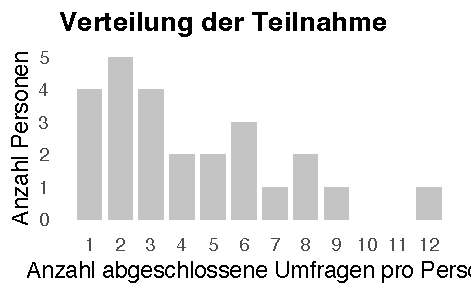
\includegraphics[width=8cm]{Analyse/Plots/survey_counts.pdf}
    \caption{Verteilung der Anzahl abgeschlossener Momentaufnahmen pro Person}
    \label{fig:survey_counts}
\end{figure}

\begin{figure}[h]
    \centering
    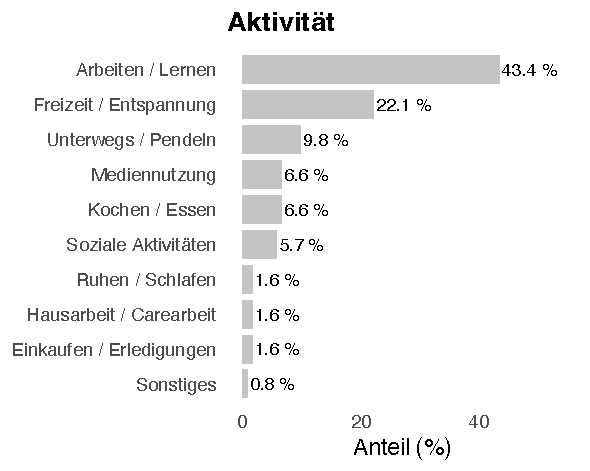
\includegraphics[width=10cm]{Analyse/Plots/cat_dist_activity.pdf}
    \caption{Tätigkeit während der Momentaufnahme}
    \label{fig:survey_activities}
\end{figure}

\begin{figure}[h]
    \centering
    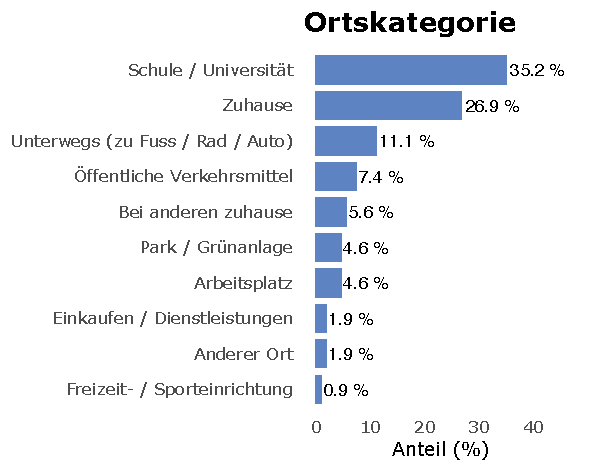
\includegraphics[width=10cm]{Analyse/Plots/cat_dist_location_category.pdf}
    \caption{Aufenthaltsortkategorie während der Momentaufnahme}
    \label{fig:survey_locations}
\end{figure}


\section{Quantitativ-intersektional analysieren -- Ein Widerspruch?}

Wie in \cref{sec:theoretischer_rahmen} dargelegt, besteht eine grundlegende Spannung zwischen den theoretischen Ansprüchen intersektionaler Forschung und den Anforderungen quantitativer Analyseverfahren. Bevor ich die Daten aus der Pilotstudie analysiere, will ich diese Spannung aufgreifen und meinen methodischen Zugang mit \gls{i-maihda} begründen.

Während Intersektionalität auf die komplexe, relationale und kontextabhängige Überlagerung sozialer Kategorien abzielt, verlangen statistische Modelle in der Regel klar definierte, operationalisierte Variablen. Damit einher geht die Gefahr, fluid-dynamische Identitäten in starre Kategorien zu übersetzen und deren soziale Konstruiertheit zu verschleiern \parencite{hancockWhenMultiplicationDoesnt2007, bowlegInvitedReflectionQuantifying2016}. Hinzu kommt, dass viele herkömmliche Verfahren additive oder eindimensionale Effekte modellieren, wodurch genau jene Interdependenzen und Wechselwirkungen nivelliert werden, die intersektionale Ansätze sichtbar machen wollen \parencite{scottIntersectionalityQuantitativeMethods2017}.

Diese methodische Spannung ist nicht nur ein technisches Problem, sondern berührt den Kern intersektionaler Forschung: Die Gefahr, sozial konstruierte Kategorien wie feste, unveränderliche Eigenschaften zu behandeln, steht im Widerspruch zu ihrem theoretischen Verständnis als zeitlich, räumlich und sozial wandelbare Konstrukte. Jede quantitative Operationalisierung muss daher reflexiv mit diesen Grenzen umgehen und das Risiko methodischer Vereinfachungen offenlegen \parencite{rodo-de-zarateDevelopingGeographiesIntersectionality2014, websterCenteringSocialtechnicalRelations2021}.

Vor diesem Hintergrund setze ich in dieser Pilotanalyse \glsxtrfull{i-maihda}\footnotemark ein. \gls{i-maihda} ist ein flexibles, mehrstufiges Analysemodell, das Daten in Gruppen („\glspl{stratum}“) verschachtelt, die sich aus der Kombination mehrerer sozialer Merkmale ergeben. Jede Person gehört genau zu einem solchen sozialen \gls{stratum}. Innerhalb eines sozialen \gls{stratum} können sich die Werte der untersuchten Variablen (\gls[noindex]{zb} (Un\nobreakdash-)Wohlbefinden) zwischen Personen unterscheiden, während sich gleichzeitig Unterschiede zwischen den sozialen \glspl{stratum} selbst zeigen.

\footnotetext{Die beiden Begriffe \emph{\glsxtrfull{maihda}} und \emph{\glsxtrfull{i-maihda}} beziehen sich auf dasselbe zugrundeliegende statistische Verfahren; die Bezeichnung mit vorangestelltem \enquote{I} hebt jedoch die intersektionale Perspektive explizit hervor und fordert die Einbettung der Analyse in einen Prozess, der theoretische Entscheidungen und methodische Vereinfachungen laufend kritisch reflektiert \parencite{evansTutorialConductingIntersectional2024}. In dieser Arbeit verwende ich deshalb den Begriff \emph{\gls{i-maihda}}, um diesen Anspruch sichtbar zu machen.}

Statistisch handelt es sich um ein hierarchisches Modell, das mindestens zwei Ebenen umfasst: \textit{Level 1} sind die einzelnen Beobachtungen, \textit{Level 2} die sozialen \glspl{stratum}. \gls{i-maihda} schätzt, wie sich die Gesamtvarianz -- also die Streuung der Messwerte im gesamten Datensatz -- auf unterschiedliche Ebenen verteilt. Dabei wird getrennt zwischen Varianz, die zwischen den sozialen \glspl{stratum} liegt, und Varianz, die innerhalb der sozialen \glspl{stratum} entsteht. Diese Zerlegung erlaubt es zu erkennen, in welchem Ausmass die Kombination sozialer Merkmale systematische Unterschiede im Outcome erklärt und wie viel der Unterschiede auf individuelle oder situative Faktoren zurückzuführen ist. In grossen Datensätzen ermöglicht dieser Ansatz die Modellierung komplexer \glspl{stratum} mit zahlreichen kombinierten Merkmalen.

Der zentrale Vorteil von \gls{i-maihda} gegenüber klassischen Regressionsmodellen liegt darin, dass nicht nur einzelne Haupteffekte und ausgewählte Interaktionsterme berücksichtigt werden, sondern jede Merkmalskombination als eigenständige Analyseeinheit behandelt wird \parencite{scottIntersectionalityQuantitativeMethods2017,bowlegInvitedReflectionQuantifying2016}. Zudem ermöglicht \gls{i-maihda} die Berechnung der sogenannten \enquote{diskriminatorischen Genauigkeit} -- ein Mass dafür, wie trennscharf die gewählten sozialen \glspl{stratum} das Outcome im jeweiligen Kontext erklären \parencite{evansTutorialConductingIntersectional2024}.

\gls{i-maihda} ist aus der epidemiologischen Mehrebenenanalyse hervorgegangen und wurde nicht primär entwickelt, um intersektionale Theorien oder Machtverhältnisse theoretisch zu adressieren. Seine intersektionale Anschlussfähigkeit entsteht erst durch eine bewusste, theoriegeleitete Auswahl der Merkmale, eine reflektierte Modellierung und die Einbettung der Ergebnisse in einen sozialen und politischen Kontext \parencite{grossModellingIntersectionalityQuantitative2023}. In diesem Sinne kann \gls{i-maihda} helfen, die eingangs skizzierte Spannung zwischen theoretischem Anspruch und quantitativer Operationalisierung zu verringern -- sie jedoch nicht vollständig auflösen.

\section{Versuch einer Analyse}

Mit dieser Pilotanalyse will ich prüfen, ob und in welchem Ausmass sich Unterschiede im situierten (Un\nobreakdash-)Wohlbefinden durch die Kombination mehrerer sozialer \glspl{stratum} und durch situative Kontextfaktoren erklären lassen. Dafür setze ich ein mehrstufiges Analyseverfahren ein, das die Messwerte auf verschiedenen Ebenen der Datenhierarchie modelliert. Da die Stichprobe klein und unbalanciert ist -- viele \glspl{stratum} umfassen nur eine Person und die Zahl der Befragungen pro Person ist gering -- verstehe ich die folgenden Schritte als methodische Illustration und nicht als inhaltlich belastbare Beantwortung der Forschungsfrage. Im Analysevorgehen folge ich \textcite{evansTutorialConductingIntersectional2024}.

Als abhängige Variable verwende ich einen Wohlbefindensindex, den ich aus fünf Einzelfragen bilde: Generelles Wohlbefinden, aktuelle Zufriedenheit, vorhandene Anspannung, Energie und soziale Zugehörigkeit (Die genaue Formulierung der Fragen und die Verteilung der Antworten ist in \cref{app:slider_hists} festgehalten). Alle Items sind auf einen Wertebereich von $0$ bis $1$ skaliert, wobei höhere Werte stets ein positiveres Befinden darstellen. Anschliessend aggregiere ich die Items mittels des geometrischen Mittels, um zu vermeiden, dass ein sehr hoher Wert in einer Dimension einen niedrigen Wert in einer anderen vollständig ausgleicht; zugleich reduziere ich dadurch den Einfluss einzelner Ausreisser.

Als zeitinvariante erklärende Variablen verwende ich die vier \glslink{identitaetsachse}{Achsen} \emph{\gls[noindex]{gender}}, \emph{Altersgruppe}, \emph{sexuelle Orientierung} und \emph{Äquivalenzeinkommensgruppe} (\gls{vgl} \cref{tab:soziodemografie_gesamt}). Die eindeutige Kombination dieser Merkmale definiert ein soziales \gls{stratum}. Damit gehört jede Person genau zu einem solchen \gls{stratum}.

Die zeitvariablen Kontextmerkmale beziehen sich auf die jeweilige Situation der Momentaufnahme und umfassen Aufenthaltsort (Innen- oder Aussenraum, spezifische Ortskategorie), Anwesenheit und Art der Beziehung zu anderen Personen, Hauptaktivität, Mehrheitsvergleich sowie vier metrische Bewertungen der Umgebung: wahrgenommene Lautstärke, sichtbare Natur, Lebhaftigkeit und empfundene Angenehmheit (\gls{vgl} \cref{tab:moments,app:slider_hists}).

Kategoriale Variablen kodiere ich als Dummy-Variablen, wobei jeweils eine Referenzkategorie entfällt, um die statistische Identifizierbarkeit sicherzustellen. Um personenspezifische Verschiebungen herauszurechnen und intraindividuelle Abweichungen vom persönlichen Mittelwert sichtbar zu machen, zentriere ich die vier metrischen Umweltbewertungen nach dem \emph{person-mean}-Verfahren, indem ich von jeder Beobachtung den individuellen Durchschnittswert der jeweiligen Person abziehe. Ein positiver Wert zeigt an, dass eine Situation lauter, naturreicher, lebhafter oder angenehmer erlebt wird als für diese Person gewöhnlich. Dieses Vorgehen trennt kurzfristige Schwankungen innerhalb einer Person von stabilen Unterschieden zwischen Personen.

\subsection*{Modellbildung}

Das erste Modell ($M0_{3L}$) dient dazu, die Gesamtvarianz des Wohlbefindens auf die verschiedenen Ebenen zu zerlegen. Die Ebenen sind:

\begin{enumerate}
    \item \emph{Level~1:} einzelne Momentaufnahmen,
    \item \emph{Level~2:} Personen,
    \item \emph{Level~3:} soziale \glspl{stratum}.
\end{enumerate}

\footnotesize
\begin{longtable}{llll ccc}
    \caption{Übersicht über soziale \glspl[noindex]{stratum}}\label{tab:strata-uebersicht}\\
    \toprule
    Geschl. & Alter & Sex. Orient. & Äquiv.-Eink. & Pers. & Befr. & Befr./Pers.\\
    \midrule
    \endfirsthead
    
    \multicolumn{7}{c}{{Tabelle \thetable{} -- Fortsetzung}} \\
    \toprule
    Geschl. & Alter & Sex. Orient. & Äquiv.-Eink. & Pers. & Befr. & Befr./Pers.\\
    \midrule
    \endhead
    
    \midrule
    \multicolumn{7}{r}{Fortsetzung auf der nächsten Seite}\\
    \endfoot
    
    \bottomrule
    \endlastfoot
    
    weiblich    & 16 -- 25    & heterosexuell & Hoch           & 3 & 13 & 4.33 \\
    männlich    & 16 -- 25    & heterosexuell & Sehr niedrig   & 3 &  9 & 3.00 \\
    männlich    & 16 -- 25    & heterosexuell & \textemdash    & 2 &  9 & 4.50 \\
    weiblich    & 16 -- 25    & heterosexuell & \textemdash    & 2 &  8 & 4.00 \\
    weiblich    & 16 -- 25    & bisexuell     & \textemdash    & 1 & 12 & 12.00\\
    männlich    & 16 -- 25    & heterosexuell & Sehr hoch      & 1 &  9 & 9.00 \\
    männlich    & 16 -- 25    & heterosexuell & Niedrig        & 1 &  8 & 8.00 \\
    männlich    & 16 -- 25    & homosexuell   & Niedrig        & 1 &  7 & 7.00 \\
    weiblich    & 16 -- 25    & heterosexuell & Sehr niedrig   & 1 &  6 & 6.00 \\
    weiblich    & 26 -- 35    & heterosexuell & Sehr niedrig   & 1 &  5 & 5.00 \\
    männlich    & 26 -- 35    & heterosexuell & Sehr hoch      & 1 &  4 & 4.00 \\
    männlich    & 16 -- 25    & homosexuell   & Hoch           & 1 &  3 & 3.00 \\
    männlich    & 16 -- 25    & heterosexuell & Hoch           & 1 &  3 & 3.00 \\
    männlich    & 16 -- 25    & homosexuell   & \textemdash    & 1 &  3 & 3.00 \\
    männlich    & 16 -- 25    & bisexuell     & Sehr niedrig   & 1 &  2 & 2.00 \\
    weiblich    & 16 -- 25    & queer         & Sehr niedrig   & 1 &  2 & 2.00 \\
    \textemdash & \textemdash & \textemdash   & \textemdash    & 1 &  2 & 2.00 \\
    männlich    & 26 -- 35    & bisexuell     & Sehr niedrig   & 1 &  1 & 1.00 \\
    
\end{longtable}
\normalsize


Die Schätzungen des Modells zeigen, dass rund \SI{8.9}{\percent} der Gesamtvarianz zwischen den \glspl{stratum} liegt, während sich auf der Personenebene keine eigenständige Varianz identifizieren lässt. Mit anderen Worten: Innerhalb desselben \glspl{stratum} unterscheiden sich die mittleren Wohlbefindenswerte der einzelnen Personen in meinen Daten nicht systematisch. Der Grossteil der Varianz ($\approx$\SI{91.1}{\percent}) entfällt auf kurzfristige Schwankungen zwischen verschiedenen Momentaufnahmen derselben Person.

Diese fehlende Varianz auf der Personenebene ist eine direkte Folge meiner Datenstruktur: Viele \glspl{stratum} bestehen nur aus einer einzelnen Person, und auch bei den übrigen \glspl{stratum} liegt nur eine geringe Zahl an Wiederholungsmessungen pro Person vor. Unter diesen Bedingungen kann das Modell keine stabilen Unterschiede zwischen Personen desselben \gls{stratum} identifizieren. Eine dreistufige Modellierung ist daher hier nicht sinnvoll. Für die folgenden Schritte reduziere ich deshalb das Modell auf eine zweistufige Struktur:

\begin{itemize}
    \item \emph{Level~1:} Momentaufnahmen,
    \item \emph{Level~2:} \glspl{stratum}.
\end{itemize}

Auch das zweistufige Nullmodell $(M0_{2L})$ ergibt für die sozialen \glspl{stratum} einen \gls{icc} von $\approx$\SI{8.9}{\percent}. Damit lassen sich knapp neun Prozent der Unterschiede im situativen Wohlbefinden auf systematische Differenzen zwischen den sozialen \glspl{stratum} zurückführen.

Im nächsten Schritt $(M1_{2L})$ nehme ich die vier \glspl{identitaetsachse} (\gls[noindex]{gender}, \emph{Altersgruppe}, \emph{sexuelle Orientierung}, \emph{Äquivalenzeinkommen}) als additive Haupteffekte in das Modell auf. Auf diese Weise kann ich den Anteil der Unterschiede bestimmen, der durch die Einzeleffekte dieser Variablen erklärbar ist. Da ich Wechselwirkungen zwischen den \glslink{identitaetsachse}{Achsen} dabei nicht berücksichtige, bleibt die darüber hinausgehende Varianz auf der Stratum-Ebene bestehen. Diese Restvarianz wird als \emph{intersektionaler Überschuss} bezeichnet.

In diesem Modell beträgt die Reduktion der Varianz zwischen den sozialen \glspl{stratum} eine \gls{pev} von \SI{63}{\percent}. Somit lassen sich etwa zwei Drittel der gruppenbezogenen Unterschiede durch die additiven Effekte der vier Achsen erklären; der verbleibende Anteil von rund einem Drittel beruht ausschliesslich auf deren spezifischer Kombination und stellt den intersektionalen Überschuss dar.

Im dritten Modell $(M2_{2L})$ nehme ich zusätzlich die situativen Kontextvariablen auf. Die geschätzte Varianz zwischen den sozialen \glspl{stratum} sinkt dadurch nahezu auf Null, und auch die verbleibende Restvarianz reduziert sich deutlich. Relativ zum Nullmodell entspricht dies einer erklärten zwischenstratalen Varianz von \SI{99.9}{\percent} sowie einer erklärten Restvarianz von etwa \SI{99.3}{\percent}. Damit lassen sich die Unterschiede im Wohlbefinden zwischen den sozialen \glspl{stratum} in dieser Stichprobe nahezu vollständig durch die Kombination aus Einzelachsen und situativen Kontextfaktoren erklären. Die kleine und unbalancierte Stichprobe erlaubt jedoch keine belastbaren Signifikanztests. Die Ergebnisse sind als methodische Illustration zu verstehen und müssen vorsichtig interpretiert werden.


\subsection*{Analyse variierender Umwelteinflüsse zwischen sozialen Strata}

Die Forschungsfrage dieses Kapitels zielt darauf, zu verstehen, inwieweit sich situative Umweltfaktoren unterschiedlich auf das Wohlbefinden verschiedener sozialer \glspl{stratum} auswirken. Während die bisherigen Modelle lediglich Mittelwertsunterschiede zwischen den \glspl{stratum} abbilden (\emph{Random Intercepts}), wird dieser Schritt um \emph{Random Slopes} erweitert: Dadurch lässt sich modellieren, ob und wie stark sich die Wirkung einzelner Kontextfaktoren systematisch zwischen den sozialen \glspl{stratum} unterscheidet.

Methodisch eröffnet dieser Ansatz die Möglichkeit, \gls[noindex]{ema}- und \gls[noindex]{gema}-Daten so auszuwerten, dass nicht nur konstante Gruppenunterschiede, sondern auch unterschiedliche Sensitivitäten gegenüber situativen Einflüssen sichtbar werden. Auch hier dient dieser Schritt ausschliesslich einer methodischen Illustration der Potenzials.

Für jede der vier metrischen Umweltbewertungen (\emph{Lautstärke}, \emph{sichtbare Natur}, \emph{Lebhaftigkeit} und \emph{empfundene Angenehmheit}) schätze ich ein separates Mehrebenenmodell mit \emph{Random Slopes}. Die Umweltvariablen zentriere und standardisiere ich nach dem \emph{person-mean}-Verfahren, sodass die Koeffizienten als Veränderung des Wohlbefindens pro Anstieg um eine Standardabweichung gegenüber dem individuellen Mittelwert interpretierbar sind. In allen Modellen sind die vier sozialen \glspl{identitaetsachse} als feste Effekte enthalten, während für die jeweilige Umweltvariable eine variierende Steigung pro \gls{stratum} geschätzt wird. Aus den Modellen werden die stratum-spezifischen Steigungen mit \SI{95}{\percent}-Konfidenzintervallen extrahiert und in \cref{tab:effekte-pro-stratum} dargestellt.

\footnotesize
\begin{ThreePartTable}
    \begin{TableNotes}[flushleft]
        \item $\Delta$ Wohlbefindensindex pro Anstieg der erklärenden Variable um eine Standardabweichung.
        \item \textbf{Fett} = Effekt ist statistisch signifikant (95\%-Konfidenzintervall schliesst den Wert 0 aus).
        \item (\textemdash = unbekannt)
    \end{TableNotes}
      
    \begin{longtable}{llllr rrrr}
        \caption{Effekte pro Stratum} 
        \label{tab:effekte-pro-stratum} \\
        \toprule
        Geschl. & Alter & Sex. Orient. & Äquiv.-Eink. & Befr. & Lärm & Natur & Lebhaftigkeit & Angenehmeit \\
        \midrule
        \endfirsthead
        
        \multicolumn{9}{c}{{\bfseries Tabelle \thetable\ -- Fortsetzung}} \\
        \toprule
        Geschl. & Alter & Sex. Orient. & Äquiv.-Eink. & Befr. & Lärm & Natur & Lebhaftigkeit & Angenehmeit \\
        \midrule
        \endhead
        
        \midrule
        \multicolumn{9}{r}{{Fortsetzung auf der nächsten Seite}} \\
        \endfoot
        
        \bottomrule
        \insertTableNotes
        \endlastfoot
        
        Frau & 16 -- 25 & heterosexuell & hoch         & 13 & \textbf{0.04} & 0.04          & 0.04          & 0.04          \\
        Frau & 16 -- 25 & bisexuell     & ---          & 12 & \textbf{0.04} & 0.05          & \textbf{0.07} & \textbf{0.07} \\
        Mann & 16 -- 25 & heterosexuell & ---          &  9 & \textbf{0.05} & \textbf{0.07} & 0.06          & 0.05          \\
        Mann & 16 -- 25 & heterosexuell & sehr hoch    &  9 & \textbf{0.04} & 0.01          & 0.01          & 0.03          \\
        Mann & 16 -- 25 & heterosexuell & sehr niedrig &  9 & \textbf{0.04} & \textbf{0.07} & 0.03          & 0.03          \\
        Mann & 16 -- 25 & heterosexuell & niedrig      &  8 & \textbf{0.04} & 0.03          & 0.00          & 0.02          \\
        Frau & 16 -- 25 & heterosexuell & ---          &  8 & \textbf{0.04} & 0.02          & 0.04          & 0.03          \\
        Mann & 16 -- 25 & homosexuell   & niedrig      &  7 & \textbf{0.05} & 0.07          & 0.05          & 0.05          \\
        Frau & 16 -- 25 & heterosexuell & sehr niedrig &  6 & \textbf{0.04} & 0.05          & 0.04          & 0.04          \\
        Frau & 26 -- 35 & heterosexuell & sehr niedrig &  5 & \textbf{0.04} & 0.04          & 0.03          & 0.04          \\
        Mann & 26 -- 35 & heterosexuell & sehr hoch    &  4 & \textbf{0.04} & 0.05          & 0.04          & 0.05          \\
        Mann & 16 -- 25 & homosexuell   & hoch         &  3 & \textbf{0.04} & 0.02          & 0.02          & 0.02          \\
        Mann & 16 -- 25 & heterosexuell & hoch         &  3 & \textbf{0.04} & 0.04          & 0.03          & 0.03          \\
        Mann & 16 -- 25 & homosexuell   & ---          &  3 & \textbf{0.04} & \textbf{0.07} & 0.03          & 0.02          \\
        Mann & 16 -- 25 & bisexuell     & sehr niedrig &  2 & \textbf{0.04} & 0.03          & 0.02          & 0.02          \\
        Frau & 16 -- 25 & queer         & sehr niedrig &  2 & \textbf{0.04} & 0.04          & 0.03          & 0.04          \\
    
    \end{longtable}
\end{ThreePartTable}
\normalsize


Einzelne Effektschätzungen sind zwar statistisch signifikant (\SI{95}{\percent}-Konfidenzintervall schliesst 0 aus). Angesichts der geringen Fallzahlen pro Stratum und der unbalancierten Stichprobe lassen sich diese Resultate jedoch nicht inhaltlich belastbar interpretieren. Um Effekte und Signifikanzen verlässlich beurteilen zu können, wären umfangreichere Daten und weiterführende Analysen erforderlich. Da es mir in dieser Pilotstudie jedoch um eine methodische Illustration und nicht um eine inhaltlich abgesicherte Auswertung geht, führe ich die Analyse an dieser Stelle nicht weiter. In \cref{sec:diskussion} reflektiere ich die methodischen Konsequenzen aus dieser Analyse vertieft.

